% Chapter X

\chapter{Results} % Chapter title
\label{ch:results} % For referencing the chapter elsewhere, use \autoref{ch:name} 

This chapter is dedicated to the description of the OCT software that was developed for this thesis. This application handles the data acquisition task, controls the galvanometric system and performs real-time processing and visualization of the acquired OCT data. \\

\noindent The transversal resolution of the system described in \autoref{ch:setup} is also evaluated using the test resolution target introduced in the same chapter. \\

\noindent Finally, a series of B-scans, C-scans and \emph{en-face} images of a variety of different samples is presented. A part of these were acquired using a second SS-OCT system designed to work in the 1060 nm range. 


%----------------------------------------------------------------------------------------

\section{Data Acquisition Software}

The final component that is needed to obtain a working SS-OCT system is a computer application that handles data acquisition and image visualization. This program should be able to achieve real-time performances, enabling a low-delay video stream of cross-sectional OCT data. Ideally, the total acquisition rate of the system in terms of B-scan/s should be limited by the scanning speed of the galvanometric mirrors and not by the OCT software. In fact, given the transversal resolution of the system, the FOV of the scanning lens and the spot size on the focal plane, there exists a maximum frequency at which the mirrors can be driven in order to obtain distortion-free images. An extensive analysis on this matter is carried out in \cite{Calabrese2017}. \\


%Leave this chapter for the explanation of the software, technologies used, performance achieved and showcase of the measurements. B-scans, volumes and enface. Also include control of the galvo mirrors in here since it's about C++ programming. 

%Explain in detail the fact that for real time the average time to process has to be < frame time and explain buffer ring to get buffer from board using DMA. Check datasheet in the pdfviwer since there is a nice explanation of async drivers. 

\noindent The application is developed for the Windows 10 Operating System using the Object-Oriented C++ programming language, which is the only one that allows low-level memory management among those supported by the ATS9350 acquisition board. Additionally, it permits the native integration of the high performance graphics library called OpenGL\footnote{\url{https://www.opengl.org/}}. \\


The code is built using the Qt application framework\footnote{\url{https://www.qt.io/}}, which consists in a set of tools for event handling and the design of \acp{GUI}. In Qt, asynchronous code can be easily written using the Signals and Slots paradigm: when a particular event occurs, an object \emph{emits} a signal; objects that are connected to this signal will execute the appropriate slot, which is a function that takes the parameters passed by the emitted signals and perform some actions. For example, the object dealing with OCT data acquisition can emit a signal with a newly acquire B-scan, while a data visualization object connected to this signal can retrieve this data and display it without blocking the acquisition task. 

\begin{figure}[htb]
	\myfloatalign
	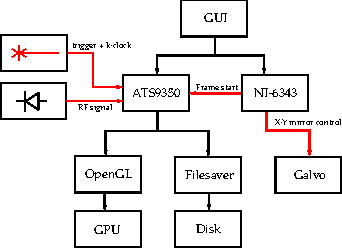
\includegraphics[width=0.6\linewidth]{gfx/ch4/dataflow}
	\caption{Data flow of the OCT application.}\label{fig:dataflow}
\end{figure}

The data flow of the application in illustrated in \autoref{fig:dataflow}. The \ac{GUI} initiates an acquisition by communicating with the ATS9350 board and an additional \ac{DAQ} board dedicated to the control of the galvo mirrors and supplying a "B-scan start" signal. This device is the National Instruments USB-6343\footnote{\url{http://www.ni.com/it-it/support/model.usb-6343.html}}, which is a USB board equipped with 4 analog outputs, 32 analog inputs and 48 digital I/O ports capable of 900 kilosamples/s. Once the ATS9350 receives the "B-scan start" signal, it will listen for A-scan triggers provided by the Axsun laser and start sampling the interference signal using the $k$-clock. After the acquisition of a B-scan is complete, the board returns a memory block containing the acquired data to the application, that will then process it and send it to two objects which asynchronously display it using OpenGL and save it to disk. 

\subsection{Controlling the galvanometric mirrors}
In order to control the galvo system, voltage signals that are proportional to the scan angle have to be sent to its driver boards. As explained in \autoref{ch:setup}, two separate signals are needed for each mirror: one for positive and one for negative angles. This requires the use of a \ac{DAQ} board with at least 4 analog output ports, explaining the choice of the USB-6434. 

To scan an area of the sample, the $X$ motor is driven with a triangle wave of frequency $f_B$ while the $Y$ motor is controlled with a "staircase" signal with a number of "steps" equal to the number of frames in the volume. At the start of each rising edge of the triangle wave, a TTL pulse will also be generated and sent to the AUX port of the ATS9350 board to signal the start of a B-scan. An example is available in \autoref{fig:galvo-signals}, where the B-scan frequency is $f_b = 20$ Hz, and the number of frames per volume is equal to 4. Using these voltages, the area that will be scanned is equal to 

\begin{equation}
	A = \left[2 EFL \tan\left( 2 \times 2 V \times 1  ^ \circ/V \times \frac{\pi}{180}\right)\right]^2 \approx 7.55\times 7.55 \text{ mm}^2.
\end{equation}
If only cross-sectional images are required, the $Y$ motor will be controlled with a constant voltage. 

During the falling edge of the triangle wave the $X$ mirror will return to its initial position, meaning that the data generated in this time interval is not useful. Hence, the number of A-scans to acquire in order to scan the entire interval covered by this mirror is

\begin{equation}\label{eq:bscan-maxwidth}
	N = \frac{1}{2} \frac{f_a}{f_b},
\end{equation}
where $f_a = 100$ kHz is the sweep repetition rate of the laser. 

\begin{figure}[htb]
	\myfloatalign
	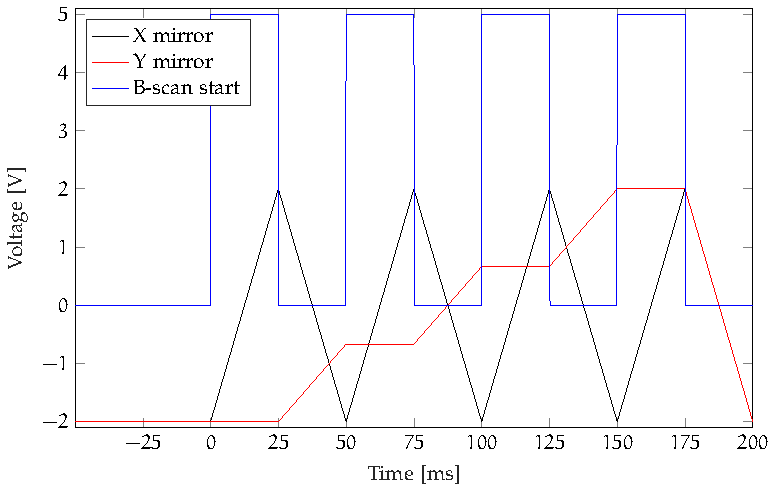
\includegraphics[width=0.9\linewidth]{gfx/ch4/galvo-signals}
	\caption{Signals used to control the galvanometric mirrors.}\label{fig:galvo-signals}
\end{figure}

Recalling that the each signal must be split in its positive and negative parts as in \autoref{eq:galvo-split-signals}, the actual signals that will be sent to the galvo driver boards will look like those in \autoref{fig:galvo-signals}.

\begin{figure}[htb]
	\myfloatalign
	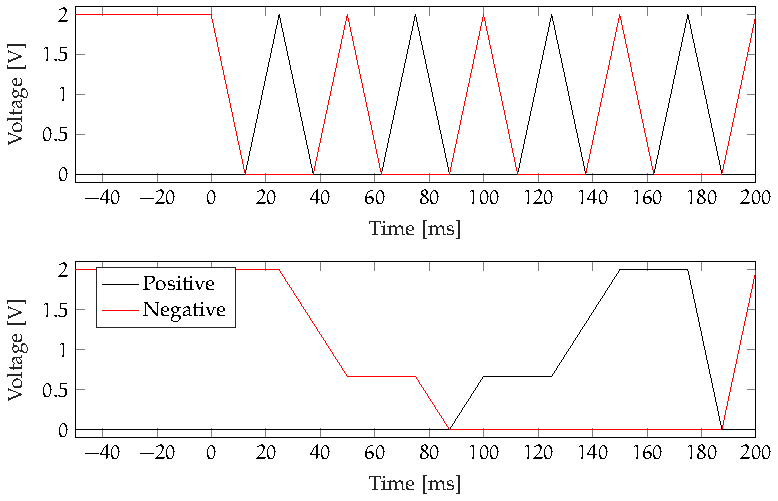
\includegraphics[width=0.9\linewidth]{gfx/ch4/galvo-signals-split}
	\caption{Signals used to control the galvanometric mirrors.}\label{fig:galvo-signals-split}
\end{figure}

\subsubsection*{Configuring the NI-6343 board}
The control of the USB-6343 board is integrated in the OCT application using the DAQmx drivers developed by National Instruments. The program is organized in \emph{tasks}; each task is a collection of channels which corresponds to a measurement or generation to perform and that can be configured independently to other tasks, specifying triggering, timing and other properties. 

In our case two tasks are created:
\begin{enumerate}
	\item Digital Task: handles the generation of the "Frame start" signal. It consists in a single digital channel which can be configured as a "digital pulse" with the \texttt{DAQmxCreateCOPulseChanFreq} function, specifying the output port of the board, the frequency of the pulse and its duty cycle. In order to generate a sequence of pulses instead of just a single one, the function \texttt{DAQmxCfgImplicitTiming} must be called to configure the task as "continuous generation". 


	
	\item Analog Task: drives the galvo system with the aforementioned signals. This task is a collection of four analog channels, which can be added with the \texttt{DAQmxCreateAOVoltageChan} command, specifying the output ports and a maximum expected voltage. 
	
	The signals are computed and stored in an array of floating point samples which will be uploaded to a buffer on the board and converted into a continuous signal by a Digital-to-Analog converter. The length of each signal is determined by the selected generation rate $R_{clk}$, the B-scan rate $f_B$ and the number of frames per volume $N_v$ as 
	\begin{equation}
		N_{\text{samples}} = R_{clk} \cdot \frac{1}{f_B} \cdot N_v,
	\end{equation}
	meaning that the length of the buffer uploaded to the board has length $4 \cdot N_{\text{samples}}$, as two analog signals are required for each mirror. Just like before, "continuous generation" must be configured, otherwise a single volume (or a single frame in case of 2D acquisition) will be scanned. To synchronize the two tasks, analog data generation is triggered by the digital pulse train created above using the \texttt{DAQmxCfgDigEdgeStartTrig} function. 
		
\end{enumerate}


\subsection{Programming the ATS9350}
In \autoref{ch:setup}, the different acquisition modes supported by the ATS9350 board were introduced. In particular, for OCT applications No-Pre-Trigger AutoDMA must be used, as it is the only method which supports high trigger repeat rates. 

Data is organized in records and buffers: records correspond to a series of samples acquired for each trigger event, while buffers are a collection of 1 or more records. In OCT, records correspond to A-scans while buffers contain a complete B-scan. 

The data transfer between the board and the software works as follows:
\begin{enumerate}
	\item A list of data buffers are allocated on the PC and assigned to the board

	\item The board will acquire the number of records necessary to fill a buffer into its main memory. 

	\item Once the records have been acquired, an AutoDMA transfer will start copying the records from the board memory to the application buffer. At the same time, the board is acquiring new records to fill the next buffer, so no trigger events are missed while copying data to the PC.

	\item After the DMA transfer is complete, the board generates an interrupt, causing an event message to be sent to the application so it can start consuming data. 
	
	\item Once the buffer has been processed by the application, it must be returned to the board. The processing time must be sufficiently low so that the board will always have one buffer available, otherwise the acquisition will fail with a BUFFER\_OVERFLOW error.
\end{enumerate}


\subsubsection{Triggering and Clocking}
Using the C++ library and headers supplied by AlazarTech, the board can be integrated in the OCT application and configured as needed. To start the acquisition of a B-scan, the AUX connector of the board is configured as "Trigger Enable In", meaning that every time a positive edge is detected on this connector the board will begin capturing a set amount of A-scans. This can be done with the following command:

\begin{lstlisting}[language=C,frame=tb]
AlazarConfigureAuxIO(boardHandle, AUX_IN_TRIGGER_ENABLE, TRIGGER_SLOPE_POSITIVE);
\end{lstlisting}

To trigger the acquisition of an A-scan instead, the sweep trigger provided by the laser is connected to the external trigger port. The board provides an advanced triggering system with two separate trigger engines, called J and K, that can either be used independently or combined to generate complex trigger events. In our case, engine K is disabled and engine J is configured to generate a trigger event when the signal connected to the external port reaches $V_{trig} = 0.71$ V. This value is passed to the board as an 8-bit integer code, calculated as 
\begin{align}
	\text{trigger code} &= 128 + 127 \times \frac{\text{trigger voltage}}{\text{input range}}\\
					&= 128 + 127 \times \frac{0.71}{5} = 146.
\end{align}

\begin{lstlisting}[language=C,frame=tb]

AlazarSetTriggerOperation(
	boardHandle,
	TRIG_ENGINE_OP_J,
	TRIG_ENGINE_J,
	TRIG_EXTERNAL,
	TRIGGER_SLOPE_POSITIVE,
	triggerCode, 
	TRIG_ENGINE_K, 
	TRIG_DISABLE, 
	TRIGGER_SLOPE_POSITIVE,
	128);

\end{lstlisting}

Similarly, clocking the board with the $k$-clock is achieved by using the \texttt{AlazarSetCaptureClock} command to select the clock source and the \texttt{AlazarSetExternalClockLevel} to select the voltage level at which samples are captured.


\subsubsection{FFT module configuration}
Achieving real-time performance without the use of \ac{GPGPU} is possible only with the use of the onboard FPGA module that computes the FFT of acquired records. To configure this module, the following code snippet is used
\begin{lstlisting}[language=C,frame=tb]
AlazarFFTSetup(	fftHandle,
	CHANNEL_A,
	samplesPerAscan,
	fftLength,
	FFT_OUTPUT_FORMAT_U16_LOG,
	fftFooter,
	0,
	&bytesPerOutputRecord
);
\end{lstlisting}
where 

\begin{itemize}
	\item \texttt{CHANNEL\_A} is the channel used for data acquisition,
	\item  \texttt{samplesPerAscan} = 1536 is the number of useful sampling clocks of the $k$-clock (\autoref{tab:axsun-datasheet}).
	\item \texttt{fftLength} = 2048 is the length of the computed FFT.
	\item \texttt{FFT\_OUTPUT\_FORMAT\_U16\_LOG} is the format in which FFT data is returned to the application, meaning that an FFT sample is computed in logarithmic scale and stored in an unsigned 16-bit integer.
	\item \texttt{bytesPerOutputRecord} is the size of an FFT record, which in this case is equal to 2 $\times$ \texttt{fftLength} = 4096 bytes.
\end{itemize}

This means that setting a B-scan frequency $f_b$, the size of a buffer is given by
\begin{equation}\label{eq:bytesperbuffer}
	\texttt{bytesPerBuffer} = \frac{1}{2} \frac{f_a}{f_b} \cdot 4096 \text{ bytes},
\end{equation}
which for $f_b = 20$ Hz is equal to 10.24 Megabytes, corresponding to $2500$ A-scans per B-scan.\\

Additionally, the FFT module can be configured to zero-pad and multiply time domain records by a windowing function:
\begin{lstlisting}[language=C,frame=tb]
AlazarDSPGenerateWindowFunction(
	windowType, // type of window to generate
	window, // memory to store window
	samplesPerAscan, // length of the fft input
	fftLength - samplesPerAscan	// zero-padding
);

AlazarFFTSetWindowFunction(
	fftHandle,
	fftLength,
	window,
	NULL // reserved 
);
\end{lstlisting}

\subsubsection{The acquisition loop}
After determining the width of each B-scan, and consequently the buffer size, a list of buffers has to be allocated on the PC and posted to the board to be used for AutoDMA transfers. 

\begin{lstlisting}[language=C,frame=tb]
for (unsigned int i = 0; i < bufferCount; i++)
{
   U16 *buffer = (U16*)VirtualAlloc(NULL, bytesPerBuffer, MEM_COMMIT, PAGE_READWRITE);
   AlazarPostAsyncBuffer(boardHandle, buffer, bytesPerBuffer);
}
\end{lstlisting}

The application will wait for the board to fill these buffers with a B-scan by using the \texttt{AlazarDSPGetBuffer} function, which returns when a DMA transfer has completed. Once this happens, the B-scan will be converted to floating point values, copied to a new buffer to be stored on disk, and then converted to suitable format to be uploaded to the GPU and be visualized on screen. After these operations are completed, the buffer is returned to the board. 

In order to keep the GUI responsive, the following loop has to be run on a separate thread:

\begin{lstlisting}[language=C,frame=tb]
unsigned int acquiredBuffers = 0;
while (acquiredBuffers < totalBscans)
{
   int bufferIndex = acquiredBuffers % bufferCount;
   U16* buffer = bufferArray[bufferIndex];
	
   // wait for the buffer to be filled
   AlazarDSPGetBuffer(boardHandle, buffer, timeout)

   // process B-scan
   float *floatBscan = convertToFloat(buffer);
   byte *Bscan = convertToImage(floatBscan);
   
   emit saveToDisk(floatBscan);
   emit uploadToGPU(Bscan);
   
   // return buffer to the board
   AlazarPostAsyncBuffer(boardHandle, buffer, bytesPerBuffer)
}
\end{lstlisting}

To remove the complex conjugate artifacts introduced in \autoref{ch:theory}, half of the data points are dropped, reducing the number of samples of each B-scan to 
\begin{equation}
	N_{\text{samples}}^{\text{B-scan}} = \frac{1}{2} \frac{f_a}{f_b} \cdot 1024
\end{equation}

B-scans are processed using a multi-processing approach enabled by the OpenMP\footnote{\url{http://www.openmp.org/}} \ac{API}, reducing the processing time needed and minimizing the total delay. \\

The floating point values from which the image is computed are first clipped in an interval $[I_{min}, I_{max}]$ controlled through the \ac{GUI} and then mapped to a 1-byte integer with values in $[0, 255]$, enabling the user to filter out the noise floor and improve the contrast of the image. 
\begin{lstlisting}[language=C,frame=tb]
...
   if (sample > Imax)
     sample = Imax;
   if (sample < Imin)
     sample = Imin;
   float range = Imax-Imin;
   byte pixelValue = 255*(sample - Imin)/range;
...
\end{lstlisting}

Finally, the raw floating point data are sent to an object that asynchronously saves it to disk while the computed image is displayed with OpenGL. 

\subsection{Processing time and delay}
Real-time data acquisition and visualization is achieved if mean processing time of a B-scan is smaller than the time between two consecutive "frame start" signals:
\begin{equation}\label{eq:processing-limit}
	\mathbb{E}[T_p] < T_b = \frac{1}{f_b}.
\end{equation}
If this inequality is not respected the delay will grow indefinitely, regardless of the amount of buffers posted to the board. In fact, if $T_p$ is constant and smaller than $T_b$, two buffers would be sufficient, but given that the processing time is a stochastic process, allocating more buffers can prevent the board from overflowing due to external factors temporarily slowing down the processing speed, like processes with higher priority in non-real time Operating Systems. 

The average processing times were measured varying the B-scan frequency $f_b$ and the number of CPU cores used in the acquisition loop, acquiring 1000 B-scans for each scenario. As can be observed in \autoref{fig:processing-time}, the application can comfortably sustain the processing load for the entire range of framerates that was tested using just a single core. 

\begin{figure}[htb]
	\myfloatalign
	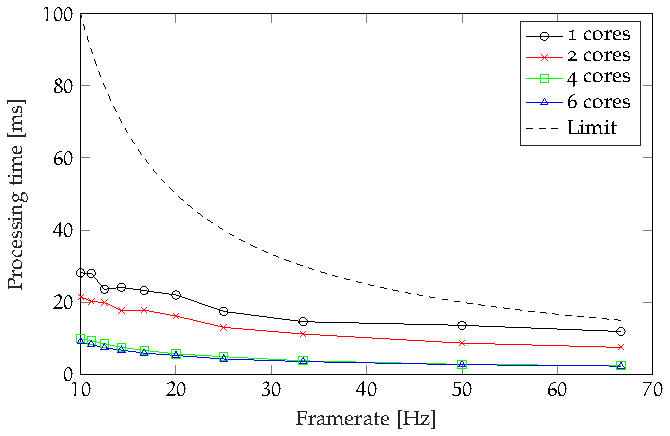
\includegraphics[width=0.8\linewidth]{gfx/ch4/processing-time}
	\caption{Processing time at different framerates and varying the number of CPU cores utilized.}\label{fig:processing-time}
\end{figure}

Even though a single core is enough to satisfy \autoref{eq:processing-limit}, using two or more is useful to reduce the total delay between the end of the acquisition of the B-scan and its visualization. This delay is computed as 
\begin{equation}
T_{\text{delay}} = T_{\text{DMA}} + T_p + T_{\text{GPU}},
\end{equation}
where $T_{\text{DMA}}$ is the time to transfer a B-scan from the ATS9350 to the application and $T_{\text{GPU}}$ is the time needed to upload the final image to the GPU and display it. Using \autoref{fig:gpu-throughput}, the DMA transfer time is computed as 

\begin{equation}
	T_{\text{DMA}} = \frac{\text{bytes per DMA buffer}}{\text{PCIe 2.0 throughput}} = \frac{\frac{1}{2}\frac{f_a}{f_b}\times 4096}{1.735 \text{ GB/s}},
\end{equation} 

where the PCIe throughput was measured in \autoref{ch:setup} using the AlazarDSO software. $T_{\text{GPU}}$ was instead measured directly inside the application. The result is visible in \autoref{fig:delay}: using 4 cores, delays shorter than 10 milliseconds are achievable even for large B-scans. 


\begin{figure}[htb]
	\myfloatalign
	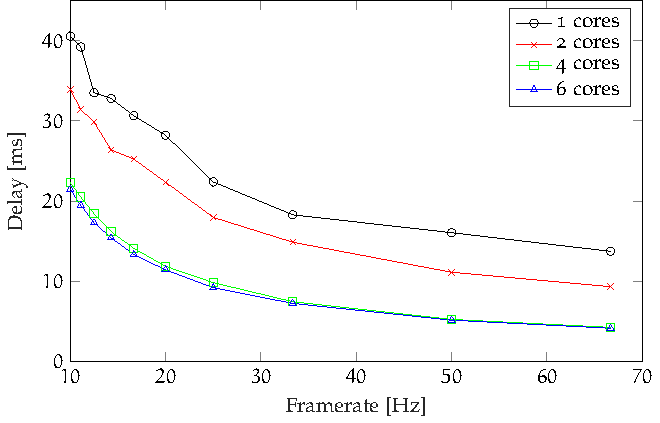
\includegraphics[width=0.8\linewidth]{gfx/ch4/delay}
	\caption{Total delay due to DMA transfer, CPU processing and GPU upload time.}\label{fig:delay}
\end{figure}

Finally, the GPU throughput is estimated as 
\begin{equation}
\eta_{\text{GPU}} = \frac{\text{bytes per image}}{\text{image upload time}} = \frac{\frac{1}{2}\frac{f_a}{f_b} \times 1024}{T_{\text{GPU}}},
\end{equation}
and illustrated in \autoref{fig:gpu-throughput}. The maximum throughput achieved by OpenGL is $\approx 9.8$ GB/s at 50 frames per second, corresponding to an image size of 1.024 MB. For lower framerates, and hence for bigger image sizes, the throughput decreases down to $7.7$ GB/s, which is about half of the theoretical maximum throughput supported by the bus. 
\begin{figure}[htb]
	\myfloatalign
	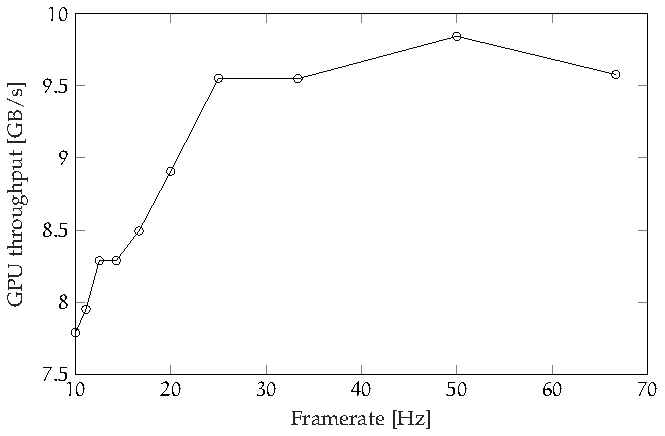
\includegraphics[width=0.8\linewidth]{gfx/ch4/gpu-throughput}
	\caption{GPU throughput using OpenGL.}\label{fig:gpu-throughput}
\end{figure}


\subsection{Saving data to disk}

\subsection{Amplified Photodiode}


\begin{figure}[hbt]
	\centering
	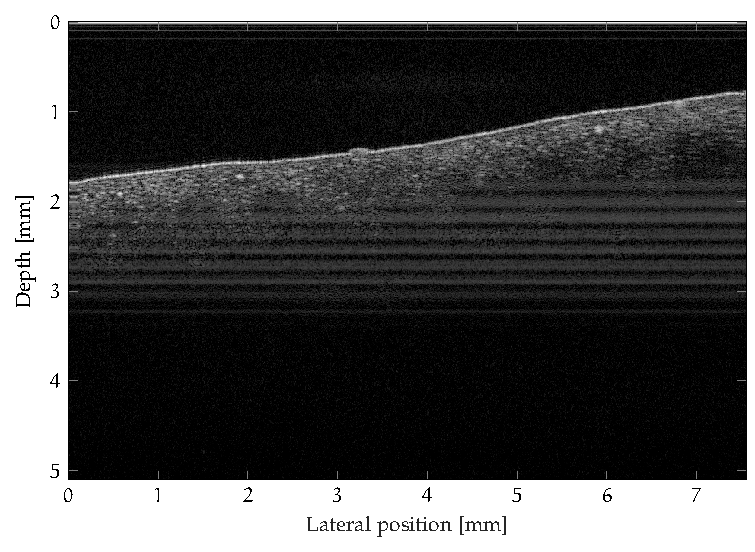
\includegraphics[width=\linewidth]{gfx/tikz/axsun/banana-peel}
	\caption{B-scan of banana peel.}\label{fig:banana-peel}
\end{figure}%----------------------------------------------------------------------------------------
\begin{figure}[hbt]
	\myfloatalign
	{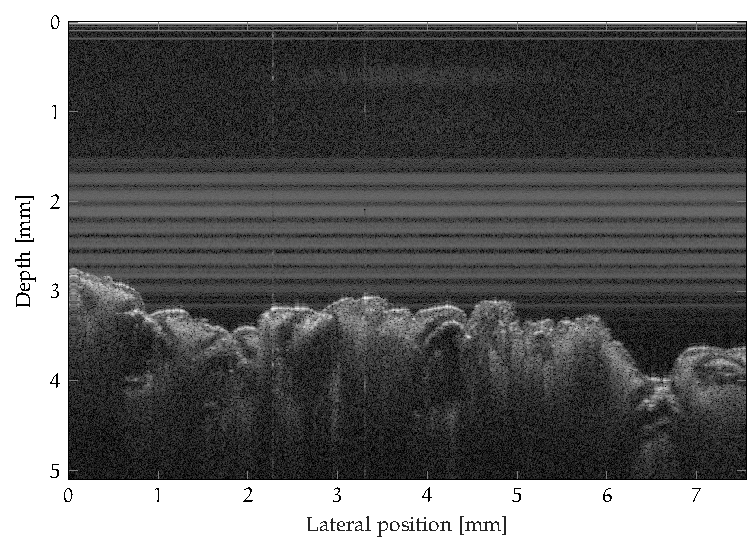
\includegraphics[width=\linewidth]{gfx/tikz/axsun/dry-orange-peel}}
	\caption{B-scan of dry orange peel.}\label{fig:dry-orange-peel}
\end{figure}%----------------------------------------------------------------------------------------

\begin{figure}[hbt]
	\myfloatalign
	{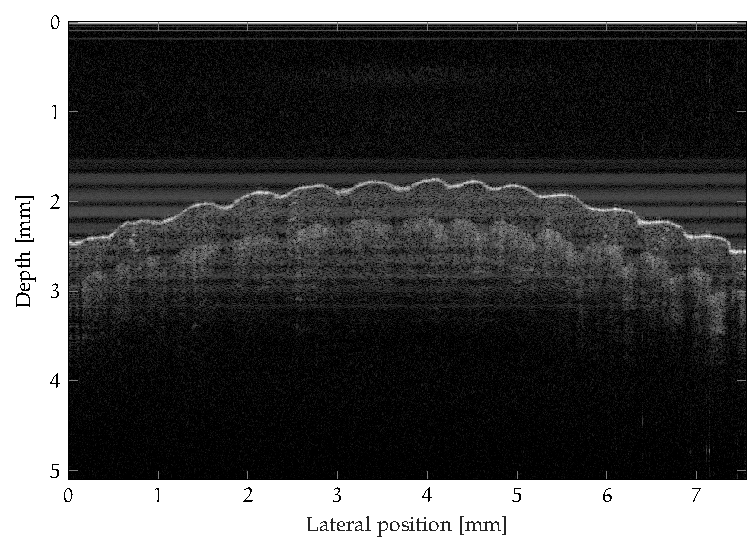
\includegraphics[width=\linewidth]{gfx/tikz/axsun/finger}}
	\caption{B-scan of a human finger.}\label{fig:finger}
\end{figure}%----------------------------------------------------------------------------------------
%----------------------------------------------------------------------------------------


\begin{figure}[hbt]
\myfloatalign
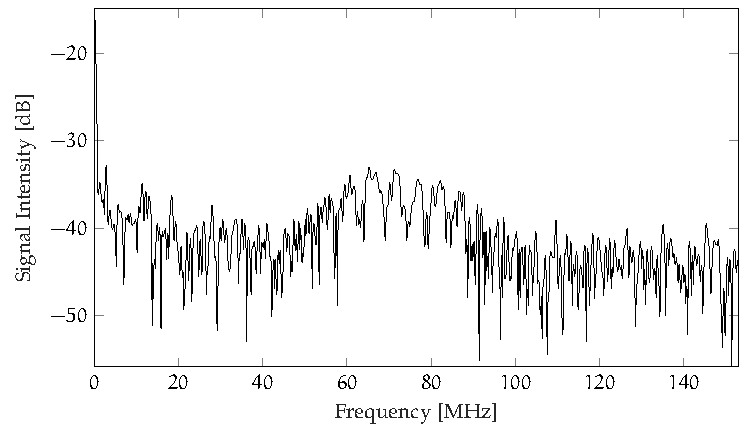
\includegraphics[width=\linewidth]{gfx/tikz/axsun/spurious-frequencies}
\caption{Spurious beat frequencies detected by the Exalos \ac{BPD}.}\label{fig:spurious-frequencies}
\end{figure}%----------------------------------------------------------------------------------------

%----------------------------------------------------------------------------------------






\begin{figure}[bth]
	\myfloatalign
	\subfloat[Asia personas duo.]
	{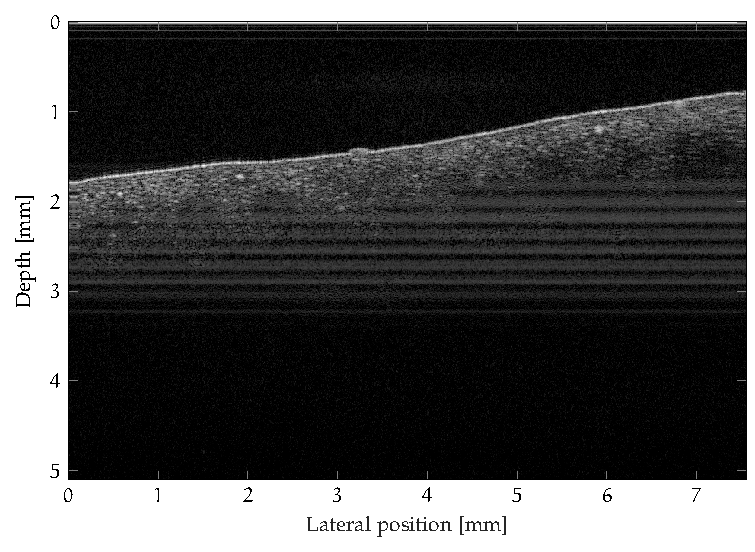
\includegraphics[width=.45\linewidth]{gfx/tikz/axsun/banana-peel}} \quad
	\subfloat[Pan ma signo.]
	{\label{fig:banan-peel}
		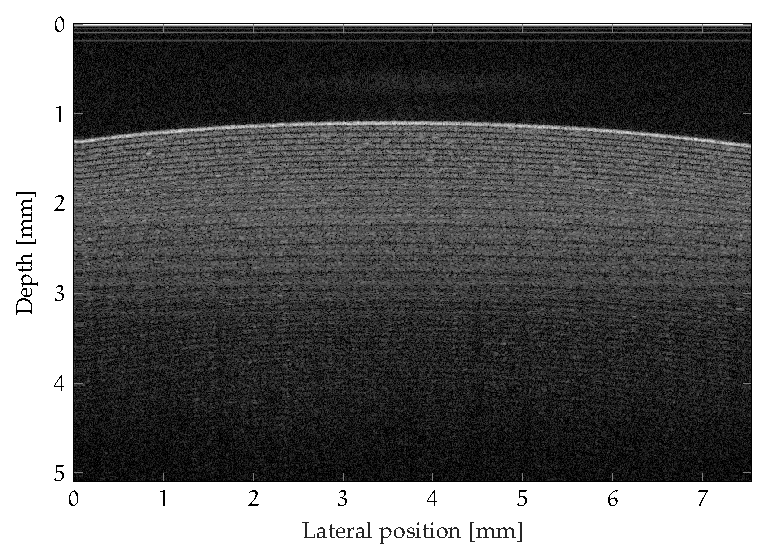
\includegraphics[width=.45\linewidth]{gfx/tikz/axsun/tape}} \\
	\subfloat[Methodicamente o uno.]
	{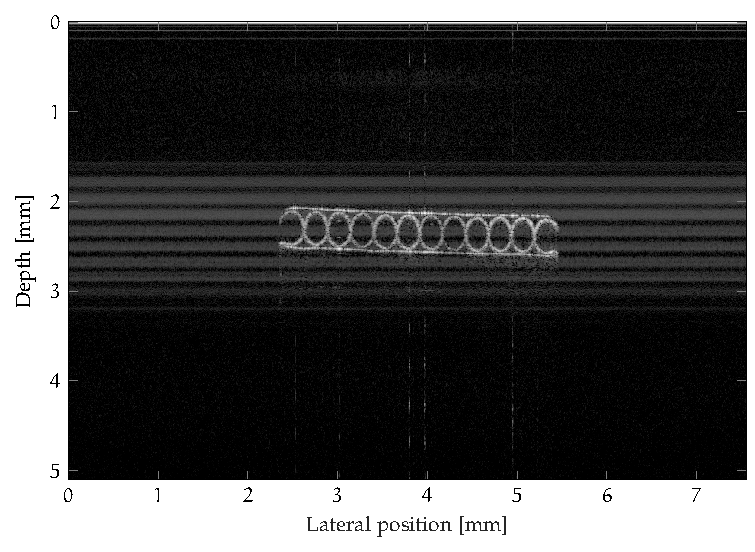
\includegraphics[width=.45\linewidth]{gfx/tikz/axsun/nastro}} \quad
	\subfloat[Titulo debitas.]
	{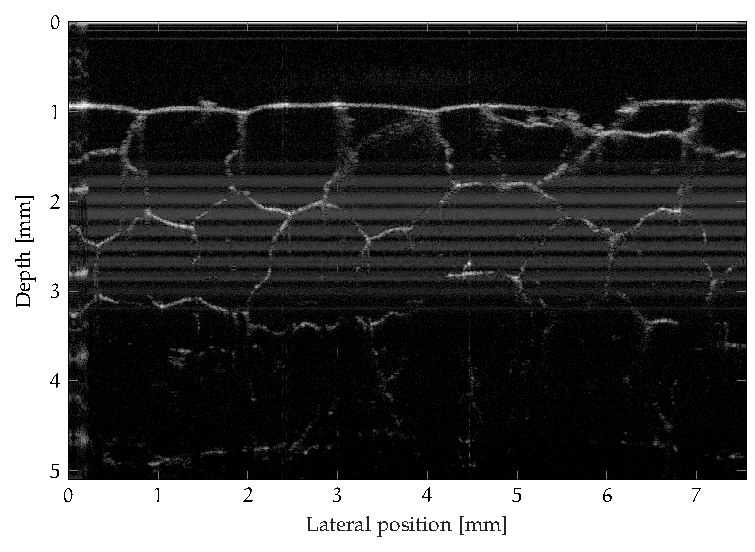
\includegraphics[width=.45\linewidth]{gfx/tikz/axsun/spugna-1}}
	\caption{Tu duo titulo debitas latente.}\label{fig:example}
\end{figure}


\section{USAF Target}
    \begin{figure}[hbt]
        \centering
        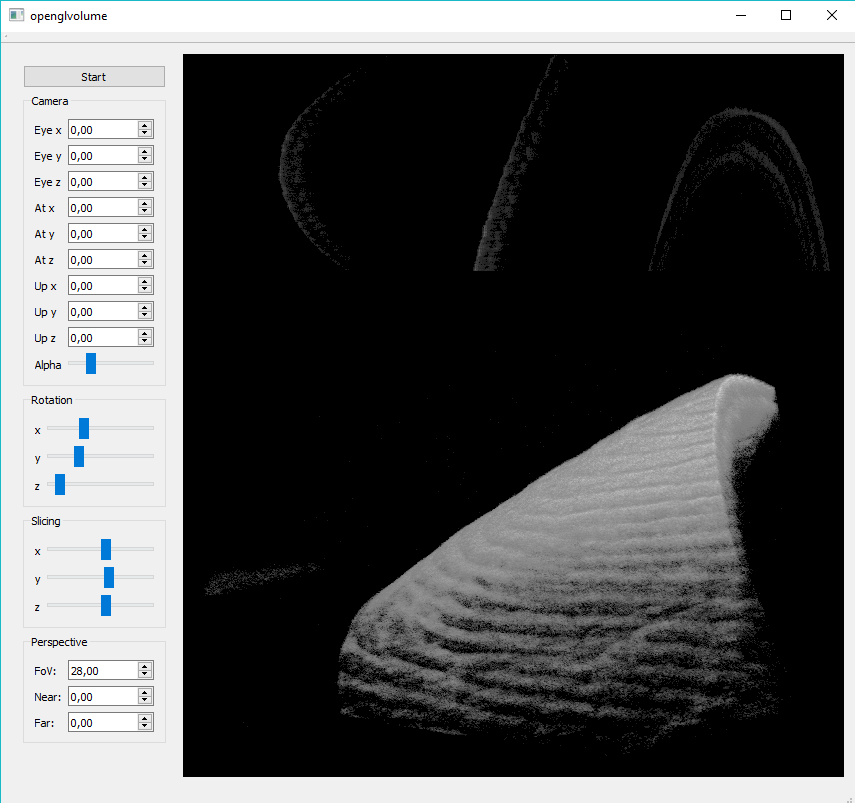
\includegraphics[width=0.8\linewidth]{gfx/3d/finger}
        \caption[]{3D rendering of a human finger.}\label{fig:finger-3d}
    \end{figure}

	\begin{figure}[hbt]
		\centering
		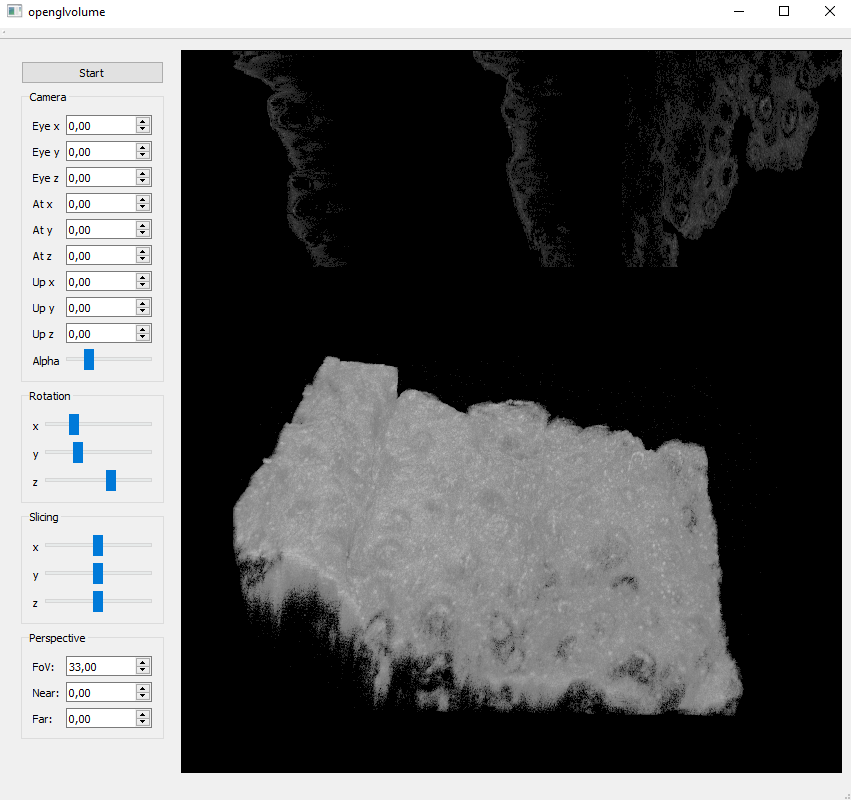
\includegraphics[width=0.8\linewidth]{gfx/3d/dry-orange}
		\caption[]{3D rendering of a human finger.}\label{fig:orange-3d}
	\end{figure}

    \begin{figure}[hbt]
        \centering
        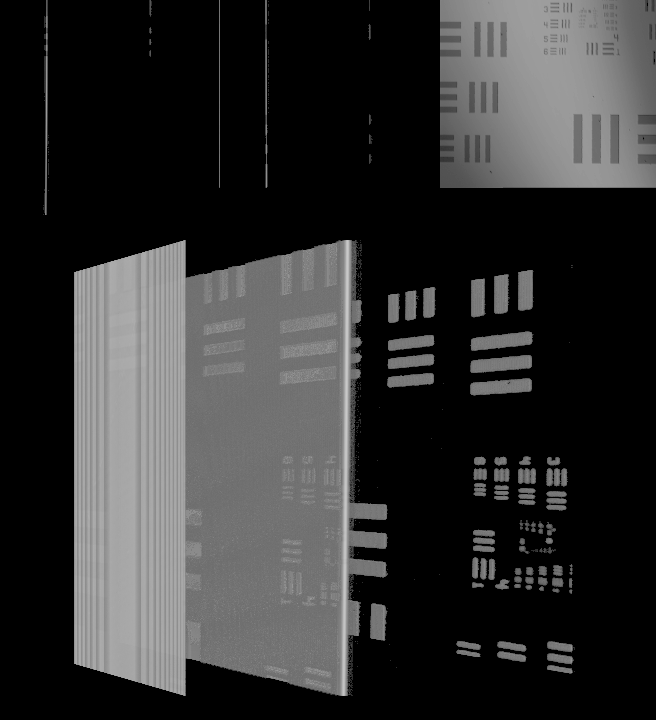
\includegraphics[width=1\linewidth]{gfx/3d/target}
        \caption[]{3D rendering of the USAF target}\label{fig:targer-3d}
    \end{figure}

	\begin{enumerate}
		\item What it is
		\item How it works
		\item Acquisitions in different conditions
		\item B-scans
		\item Surface images -> verifying transverse resolution
	\end{enumerate}

Content
